Die Konstruktion wurde in 3 einzelne Teile aufgeteilt: Bodenplatte, hinterer Aufbau und Lenkung. Diese Teile sind mit wenigen Schrauben und Steckverbindung voneinander trennbar. Dies wurde gemacht, um den Transport und die Lagerung zu vereinfachen.\\
Der Aufbau wurde in Inventor geplant und konstruiert.

\missingfigure[]{Gesamter Aufbau}

\newpage
\section{Bodenplatte}
Die Bodenplatte wurde aus 10cm dicken XPS--Platten und einer 1cm dicken Pappelsperrholzplatte zusammengesetzt. In das XPS wurden zur Verstärkung noch links und rechts 2 20x95\,mm Holzlatten eingefräst und eingeklebt.\\ 
In der Mitte der Bodenplatte wurde das Loch für den Propeller ausgeschnitten. Im XPS wurde der Lochdurchmesser so gewählt, dass der Propeller darin frei drehen kann. Der Lochdurchmesser in der Holzplatte darüber wurde um 2\,cm kleiner gewählt um zu verhindern das am Rand des Loches die Luft direkt wieder hinausströmt.

\begin{figure}[H]
    \centering
    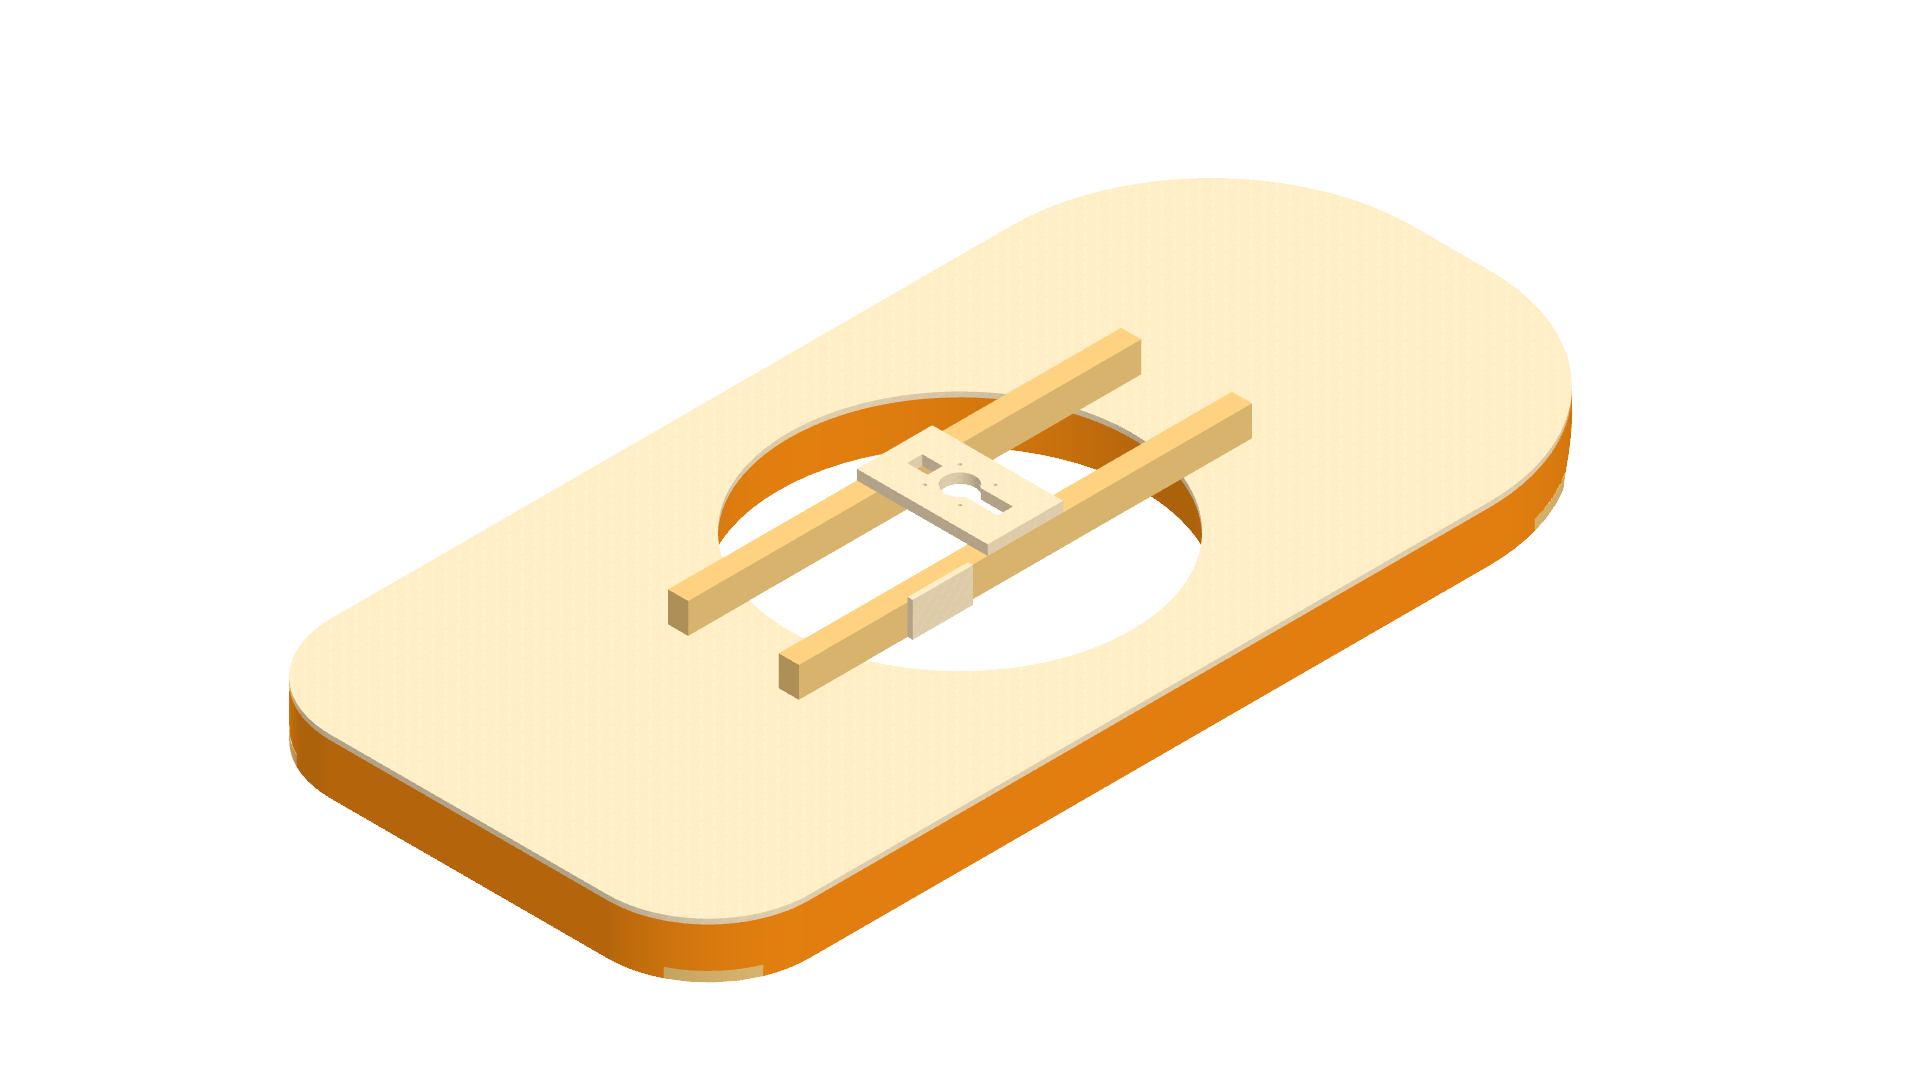
\includegraphics[width=\textwidth]{../../../../Inventor/Bodenplatte/png/BodenplatteHauptansicht.png}
    \caption{Bodenplatte 3D-Modell\label{fig:konst:bodenplatte:gesamt}}
\end{figure}

\subsection{Stückliste}
\begin{table}[H]
    \centering
    \begin{tabular}{|c|c|c|}
        \hline
        \textbf{Stk} & \textbf{Name} & \textbf{Bezeichnung}\\\hline
        1 & Bodenplatte Pappel & 10mm Pappelsperrholz\\\hline
        1 & Bodenplatte XPS & 100mm XPS\\\hline
        1 & Verstärkung Holzlatte links & Holzlatte Fichte 20x90mm\\\hline
        1 & Verstärkung Holzlatte rechts & Holzlatte Fichte 20x90mm\\\hline
        2 & Staffel Motorhalterung & Staffel gehobelt 40x60mm\\\hline
        2 & Platte Motorhalterung & 10mm Pappel\\\hline
    \end{tabular}
    \caption{Stückliste Bodenplatte}
    \label{tab:konst:bodenplatte:stueckliste}
\end{table}

\subsection{Inventor}
\begin{figure}[H]
    \centering
    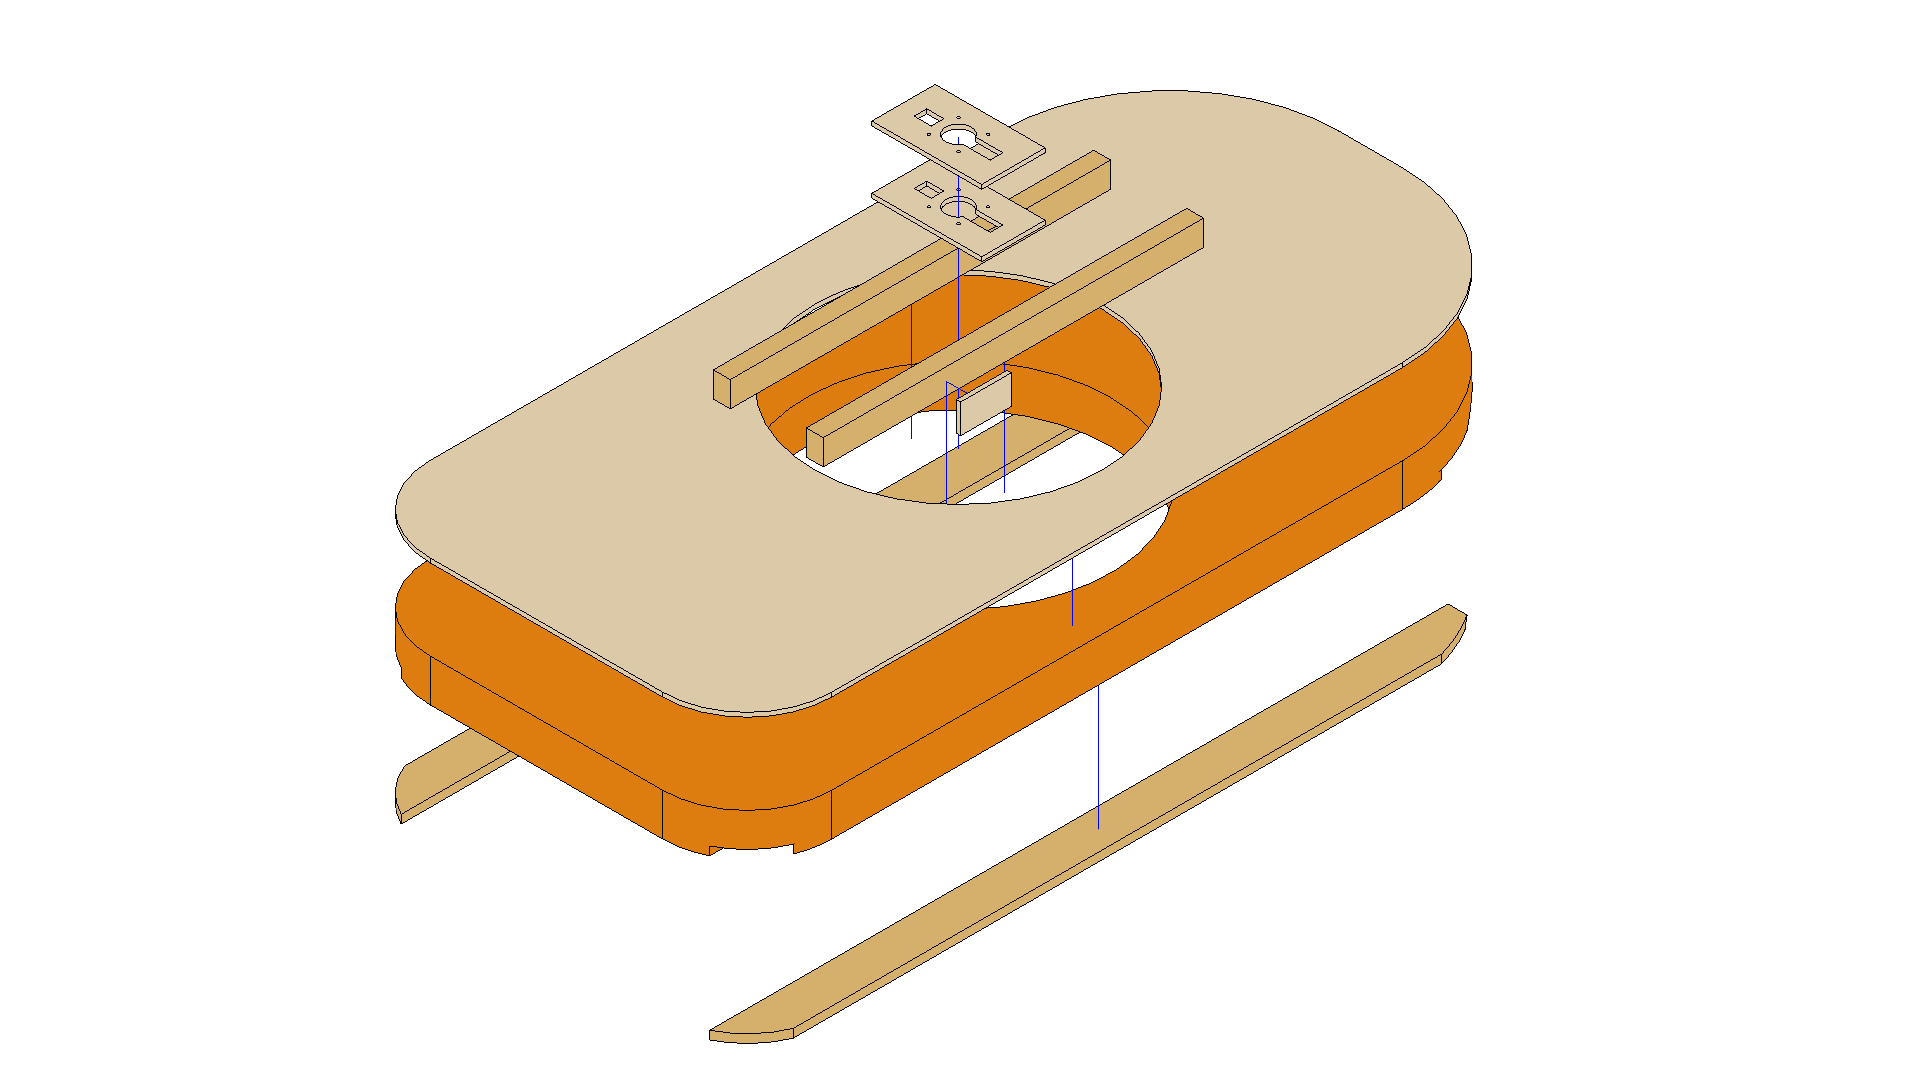
\includegraphics[width=\textwidth]{../../../../Inventor/Bodenplatte/png/Bodenplatte_Praesentation_Hauptansicht.png}
    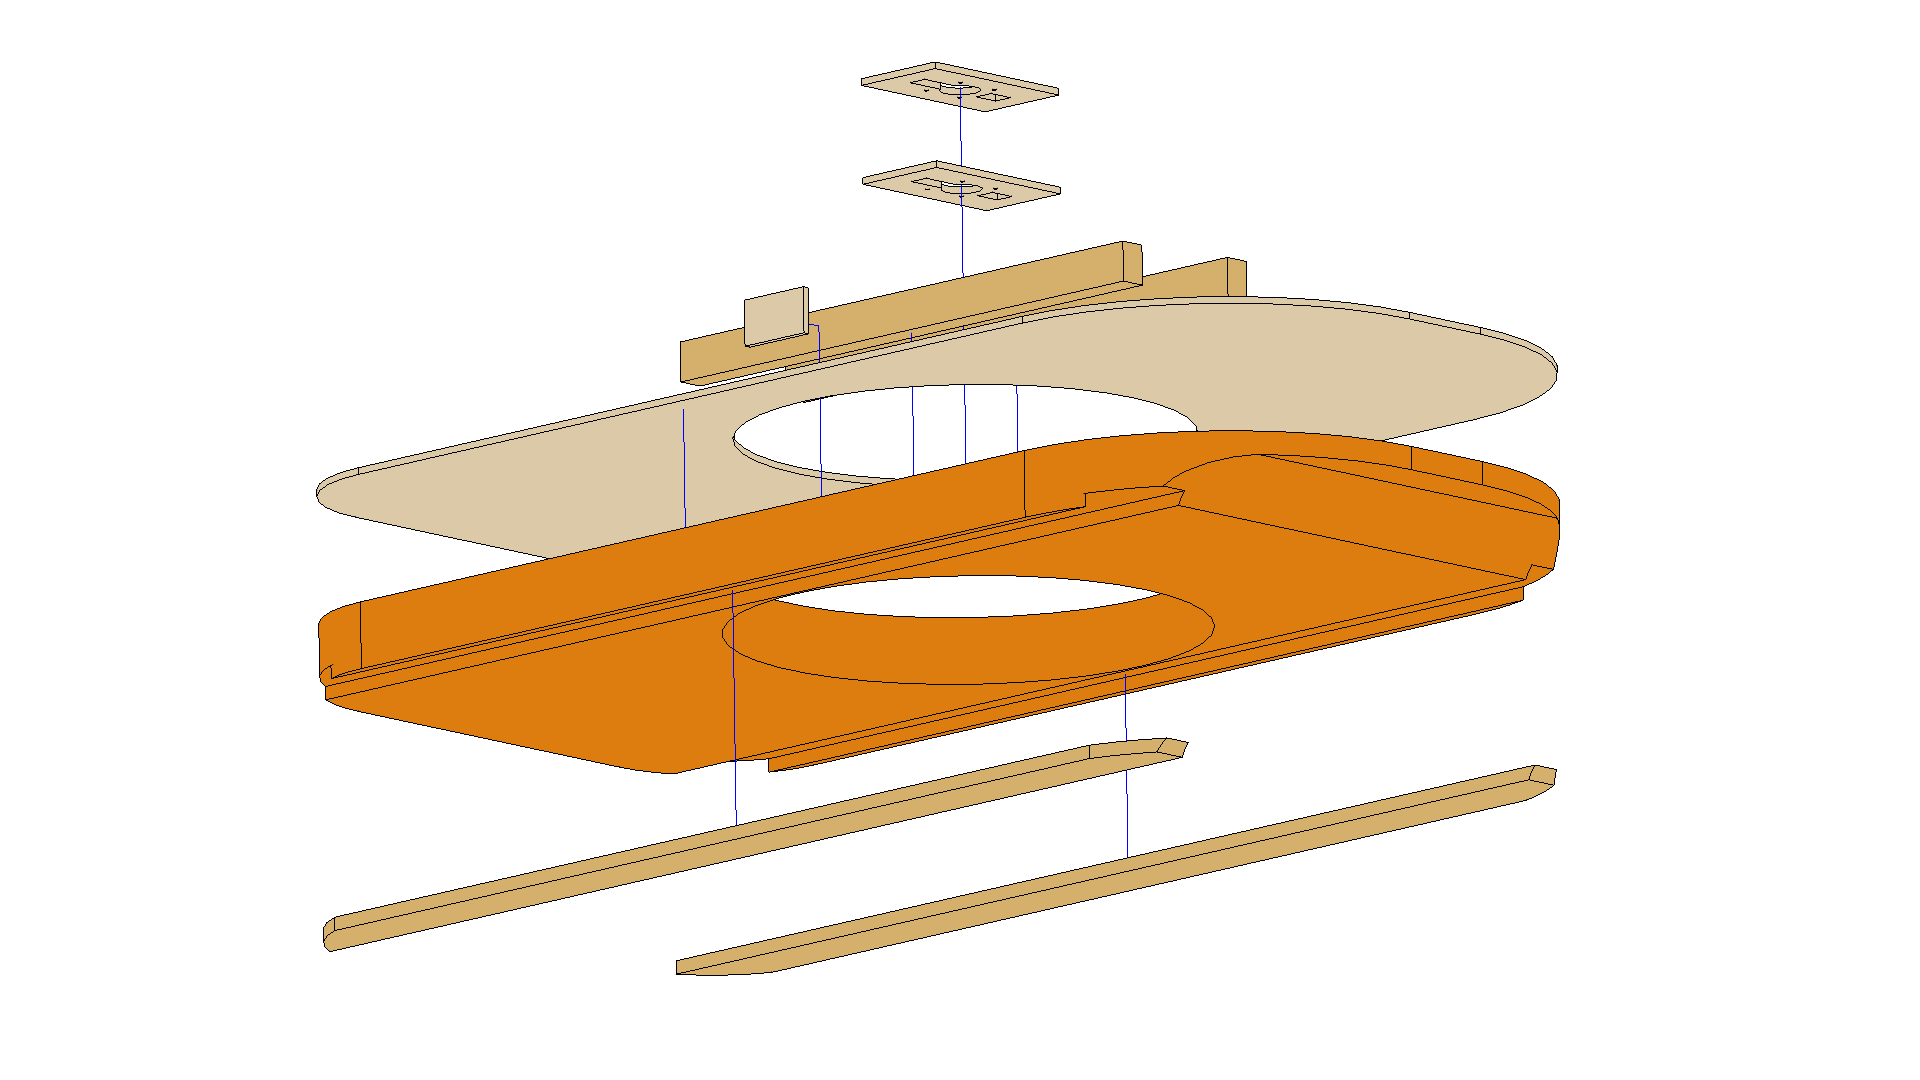
\includegraphics[width=\textwidth]{../../../../Inventor/Bodenplatte/png/Bodenplatte_Praesentation_SeitlichUnten.png}
    \label{fig:konst:bodenplatte:inventor}
    \caption{Bodenplatte Inventor Explosionsansicht}
\end{figure}
\clearpage

\begin{landscape}
    \includeSkizze{../../../../Inventor/Bodenplatte/png/Einzelteile/Bodenplatte-Holz.png}{Bodenplatte Pappel}{1}{16.02.2021}{fig:bodenplatte:skizze:BodenplattePappel}
    \clearpage

    %\includeSkizze{../../../../Inventor/Bodenplatte/png/Einzelteile/Motorhalterung.png}{Bodenplatte XPS}{1}{16.02.2021}{fig:bodenplatte:skizze:BodenplattePappel}
    %\clearpage

    \includeSkizze{../../../../Inventor/Bodenplatte/png/Einzelteile/Motorhalterung.png}{Motorhalterung}{1}{16.02.2021}{fig:bodenplatte:skizze:Motorhalterung}
    \clearpage

\end{landscape}


\cleardoublepage
\subsection{Bilder}
\missingfigure{Fotos Bodenplatte reintuen}


